%%%%%%%%%%%%%%%%%%%%%%%%%%%%%%%%%%%%%%%%%
% Fancyslides Presentation
% LaTeX Template
% Version 1.0 (30/6/13)
%
% This template has been downloaded from:
% http://www.LaTeXTemplates.com
%
% The Fancyslides class was created by:
% Paweł Łupkowski (pawel.lupkowski@gmail.com)
%
% License:
% CC BY-NC-SA 3.0 (http://creativecommons.org/licenses/by-nc-sa/3.0/)
%
%%%%%%%%%%%%%%%%%%%%%%%%%%%%%%%%%%%%%%%%%

%----------------------------------------------------------------------------------------
%	PACKAGES AND OTHER DOCUMENT CONFIGURATIONS
%----------------------------------------------------------------------------------------

\documentclass{fancyslides}

\usepackage[utf8]{inputenc} % Allows the usage of non-english characters
\usepackage{times} % Use the Times font
\usepackage{booktabs} % Allows the use of \toprule, \midrule and \bottomrule in tables
\graphicspath{{images/}} % Location of the slide background and figure files

% Beamer options - do not change
\usetheme{default} 
\setbeamertemplate{navigation symbols}{} % Disable the slide navigation buttons on the bottom of each slide
\setbeamercolor{structure}{fg=\yourowntexcol} % Define the color of titles and fixed text elements (e.g. bullet points)
\setbeamercolor{normal text}{fg=\yourowntexcol} % Define the color of text in the presentation

%------------------------------------------------
% COLORS
% The following colors are predefined in this class: white, black, gray, blue, green and orange

% Define your own color as follows:
%\definecolor{pink}{rgb}{156,0,151}

\newcommand{\structureopacity}{0.75} % Opacity (transparency) for the structure elements (boxes and circles)

\newcommand{\strcolor}{blue} % Set the color of structure elements (boxes and circles)
\newcommand{\yourowntexcol}{white} % Set the text color

%----------------------------------------------------------------------------------------
%	TITLE SLIDE
%----------------------------------------------------------------------------------------

\newcommand{\titlephrase}{Hidden Pioneers: Programmers of the ENIAC and the Birth of Modern Computing} % Presentation title
\newcommand{\name}{Nelson Jovel} % Presenter's name
\newcommand{\affil}{Education Commonwealth Project} % Presenter's institution
\newcommand{\email}{joveln@gmail.com} % Presenter's email address

\begin{document}

\startingslide % This command inserts the title slide as the first slide

%----------------------------------------------------------------------------------------
%	PRESENTATION SLIDES
%----------------------------------------------------------------------------------------

\fbckg{blank.jpg} % A blank background can be used instead of an image
\begin{frame}
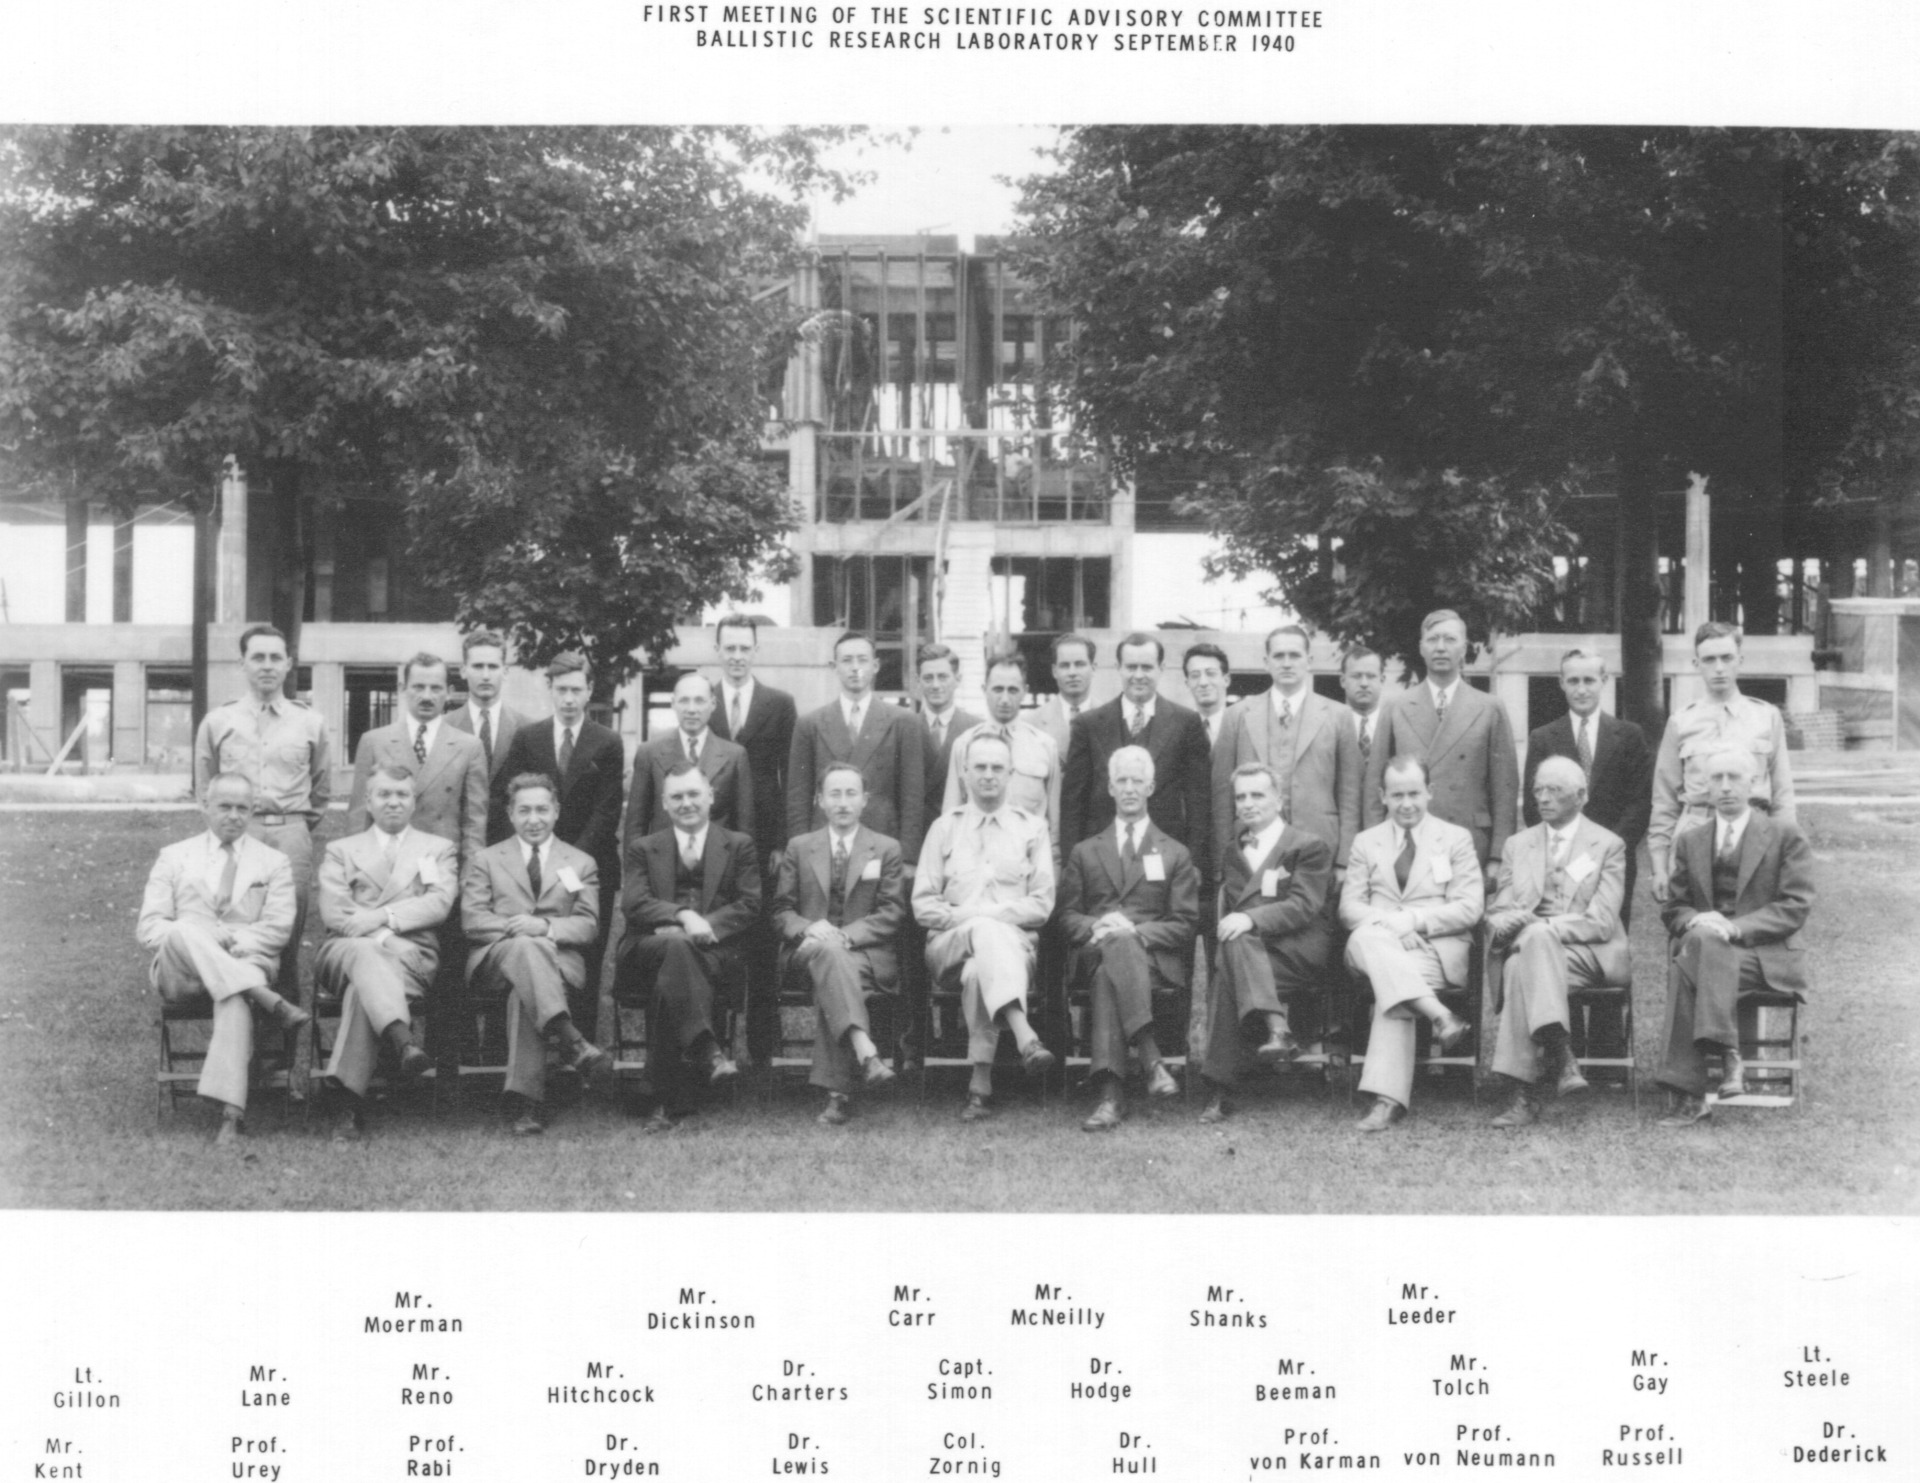
\includegraphics[scale=0.15]{ballistic_research_lab.jpg} \ US Army Ballistics Research Laboratory
\end{frame}

%------------------------------------------------

\begin{frame}
\misc{ % Anything can be placed inside the \misc{} command
Example Artillary
\begin{figure}[h]
  \begin{flushleft}Howitzer \end{flushleft} 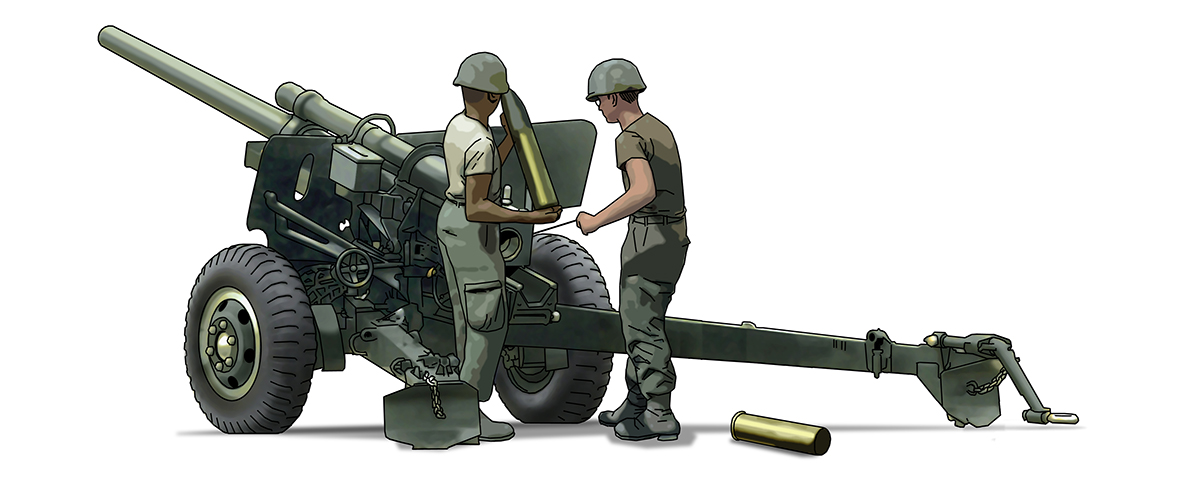
\includegraphics[width=0.25\linewidth]{howitzer_105-mm-1200_480.jpg}  \\
  \begin{flushleft}Tank \end{flushleft} 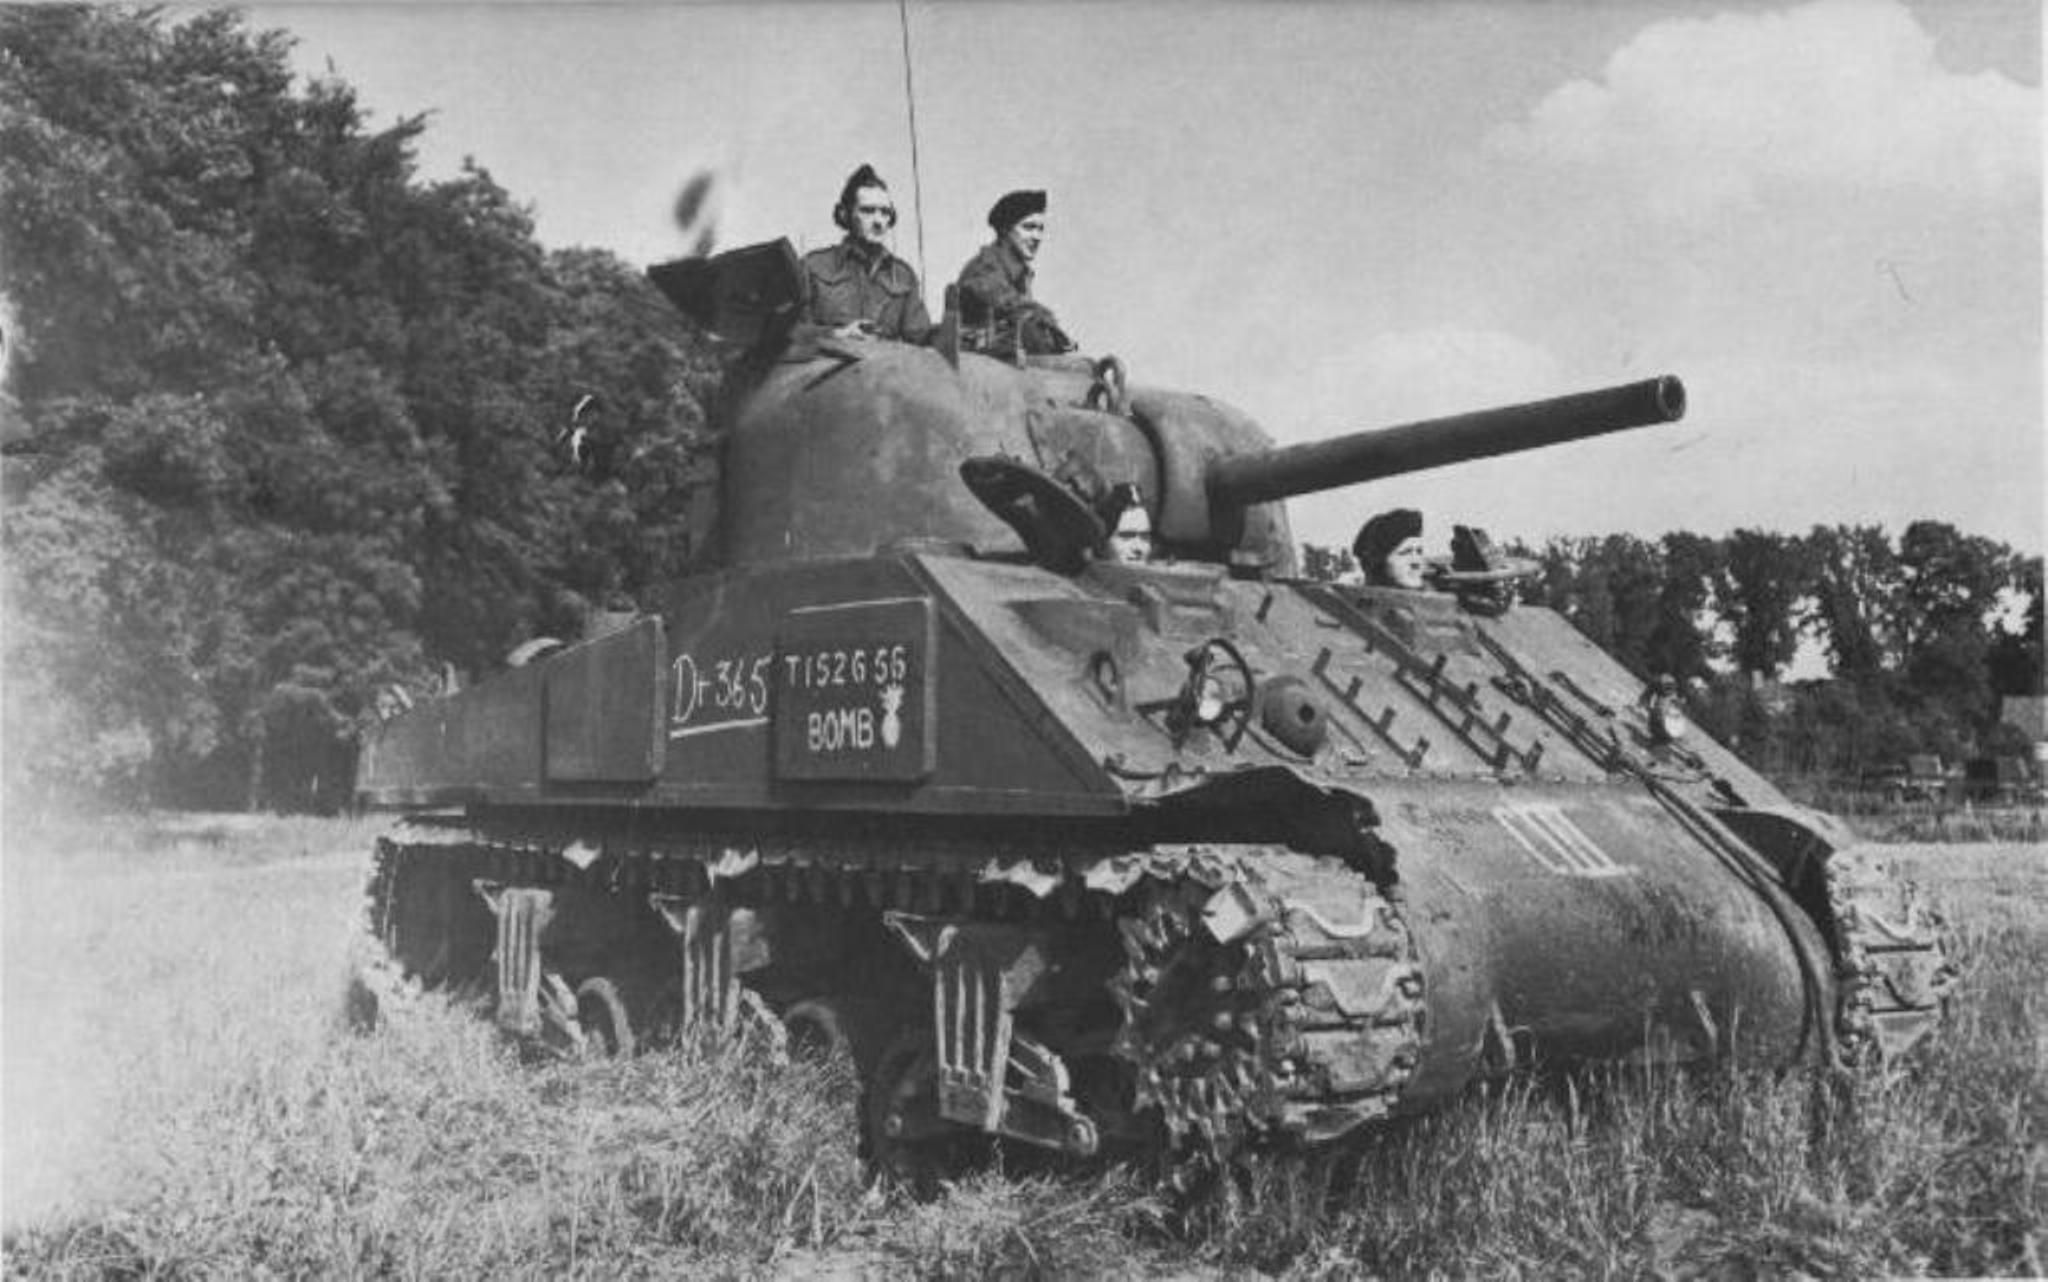
\includegraphics[width=0.2\linewidth]{m4-sherman.jpg} \\
  \begin{flushleft}Anti-Aircraft \end{flushleft} 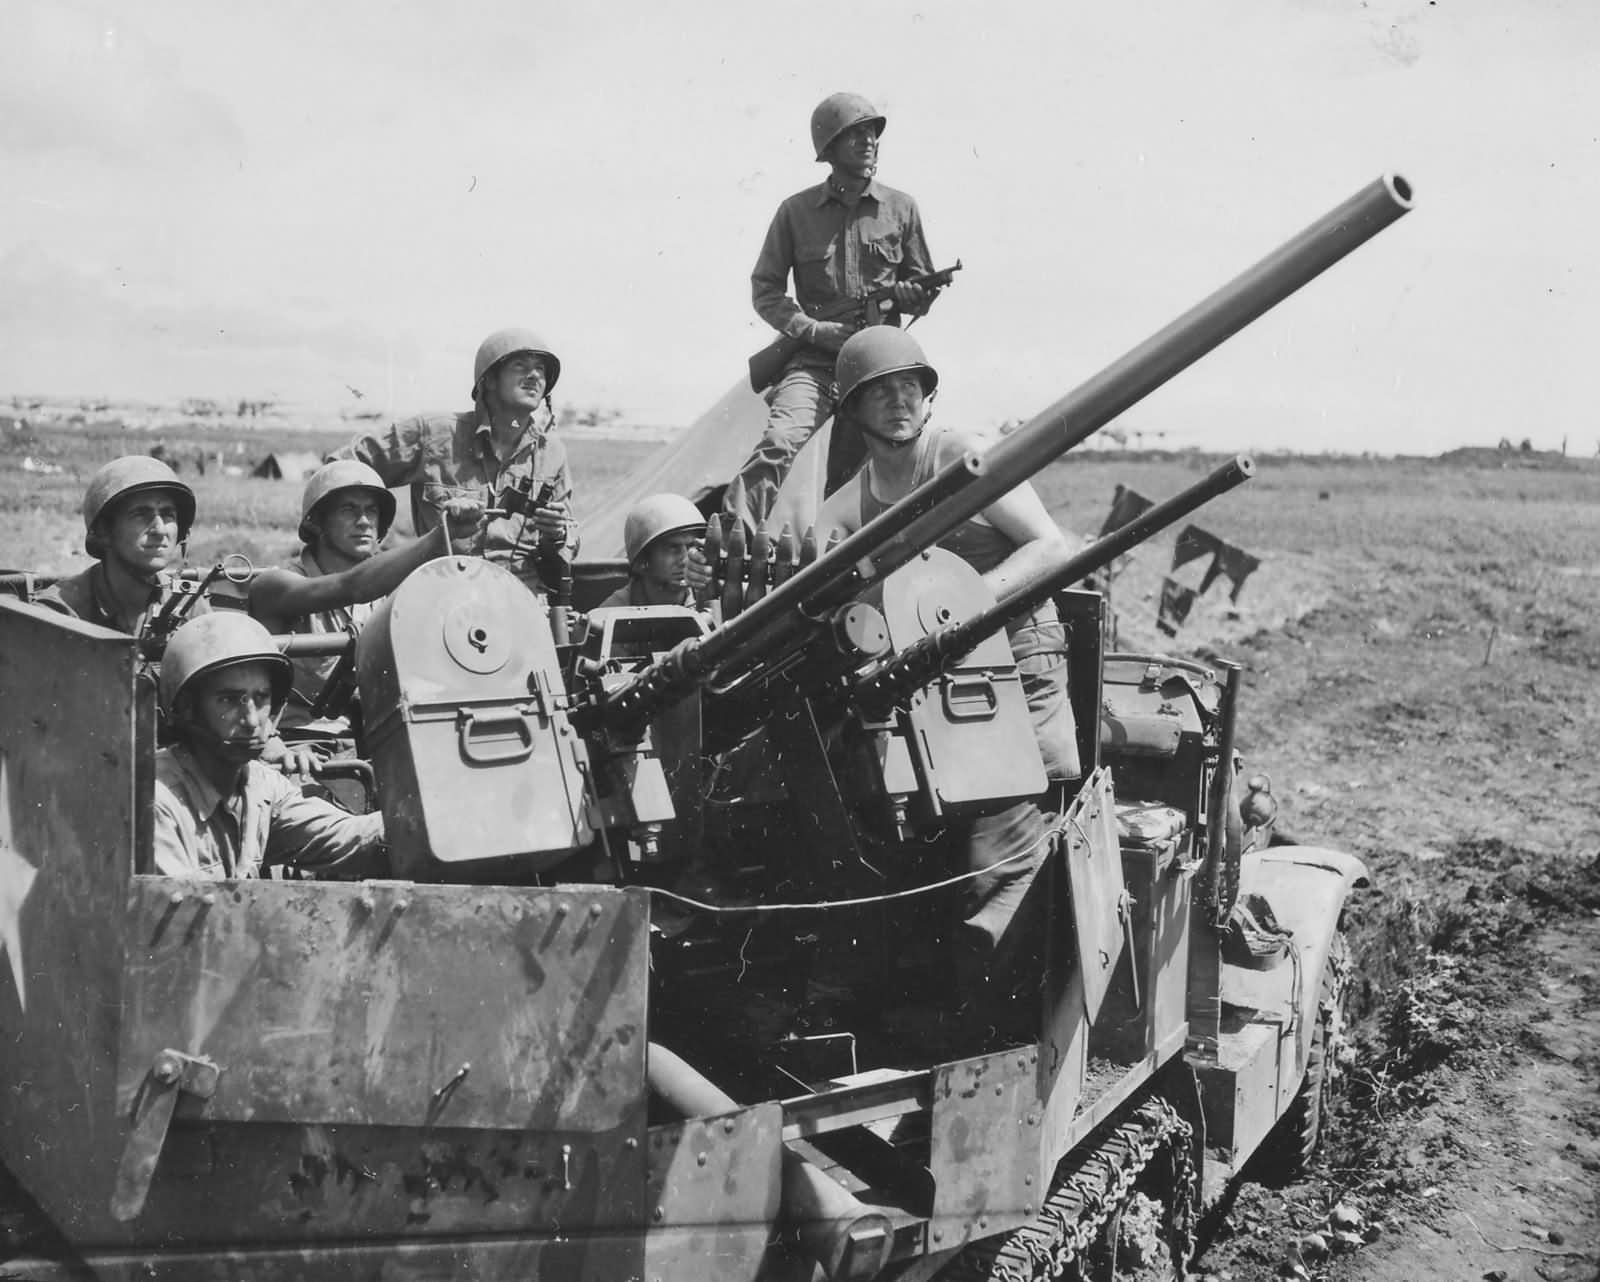
\includegraphics[width=0.2\linewidth]{Anti-Aircraft_Artillery_37mm_Halftrack_and_Thompson.jpg} \\
\end{figure}
}
\end{frame}

%------------------------------------------------

\fbckg{cannon_range_chart.jpg} % Slide background image
\begin{frame}
\text Targeting
\end{frame}

%------------------------------------------------

\fbckg{firing_table.jpg} % Slide background image
\begin{frame}
\text Targeting
\end{frame}

%------------------------------------------------

\fbckg{firing_table_rotation.jpg} % Slide background image
\begin{frame}
\end{frame}

%------------------------------------------------

\fbckg{human_computers.jpg} % Slide background image
\begin{frame}
\end{frame}


%------------------------------------------------

\fbckg{DifferentialAnalyzer.jpg} % Slide background image
\begin{frame}
  \pointedsl{Differential Analyzer}
\end{frame}

%------------------------------------------------

\fbckg{DifferentialAnalyzer.jpg} % Slide background image
\begin{frame}
\end{frame}

%------------------------------------------------

\fbckg{ww2_timeline.jpg} % Slide background image
\begin{frame}
\end{frame}

%------------------------------------------------

\fbckg{eniac_women_programmers_1.jpg} % Slide background image
\begin{frame}
\end{frame}

%------------------------------------------------

\fbckg{eniac_women_programmers_1.jpg} % Slide background image
\begin{frame}
\itemized{ % This environment simply prints a series of bullet points
  \item Designers: John Mauchley and J. Presper Eckert
}
\end{frame}

%------------------------------------------------

\fbckg{eniac_women_programmers_1.jpg} % Slide background image
\begin{frame}
\itemized{ % This environment simply prints a series of bullet points
  \item The Use of High Speed Vacuum Tube Devices for Calulating
  \item 1000 times faster than the differential analyzer
  \item General Purpose computer
}
\end{frame}

%------------------------------------------------

\fbckg{eniac_women_programmers_1.jpg} % Slide background image
\begin{frame}
\itemized{ % This environment simply prints a series of bullet points
  \item Projected Cost: 61,000
  \item Actual Cost: 500,000
  \item Today: 9,000,000+
}
\end{frame}

%------------------------------------------------

\fbckg{vacuum_tubes_history.jpg} % Slide background image
\begin{frame}
\end{frame}

%------------------------------------------------

\fbckg{vacuum_tubes_history.jpg} % Slide background image
\begin{frame}
\itemized{ % This environment simply prints a series of bullet points
  \item 18,000 Vacuum Tubes
  \item Run at lower voltages
  \item Do not power cycle
}
\end{frame}

%------------------------------------------------

\fbckg{first_four.jpg} % Slide background image
\begin{frame}
\end{frame}


%------------------------------------------------

\fbckg{first_four.jpg} % Slide background image
\begin{frame}
  \framedsl{
  \pitem{Eniac} 
  \pitem{Binac} 
  \pitem{Edvac} 
  \fitem{Univac}} 
\end{frame}

%------------------------------------------------

\fbckg{first_four.jpg} % Slide background image
\begin{frame}
  \framedsl{
  \pitem{Decimal} 
  \pitem{Modular} 
  \fitem{Linear cost to add precision} 
  } 
\end{frame}
%------------------------------------------------

\fbckg{cycling_unit.jpg} % Slide background image
\begin{frame}
  \framedsl{Engineer only what doesn't already exist}
\end{frame}

%------------------------------------------------

\fbckg{ibm_card_punch.jpg} % Slide background image
\begin{frame}
\end{frame}

%------------------------------------------------

\fbckg{ibm_card_punch.jpg} % Slide background image
\begin{frame}
  \framedsl{IBM Card Punch (80 Characters)} % Text in this environment will be made large, uppercase and will wrap multiple lines
\end{frame}

%------------------------------------------------
\fbckg{punch_card_system_3.jpg} % Slide background image
\begin{frame}
\end{frame}

%------------------------------------------------

\fbckg{5mbof-punched-card-computer-rooms.jpg} % Slide background image
\begin{frame}
\end{frame}

%------------------------------------------------

\fbckg{5mbof-punched-card-computer-rooms.jpg} % Slide background image
\begin{frame}
\framedsl{5mb of data} % Text in this environment will be made large, uppercase and will wrap multiple lines
\end{frame}

%------------------------------------------------
\fbckg{room_layout.jpg} % Slide background image
\begin{frame}
\end{frame}

%------------------------------------------------
\fbckg{room_layout.jpg} % Slide background image
\begin{frame}
\framedsl{
  \pitem{Initiating unit } 
  \pitem{Cycling unit } 
  \pitem{Master Programmer} 
  \fitem{Accumulator (20)} 
}
\end{frame}

%------------------------------------------------
\fbckg{room_layout.jpg} % Slide background image
\begin{frame}
\framedsl{
  \pitem{Divider/Square rooter -  35 per second} 
  \pitem{Multiplier - 357 multiplications per second} 
  \pitem{3 moveable function tables} 
  \pitem{Card reader} 
  \fitem{Card punch}} 
\end{frame}


%------------------------------------------------
\fbckg{eniac_women_programmers_1.jpg} % Slide background image
\begin{frame}
\itemized{ % This environment simply prints a series of bullet points
  \item Robert F. Shaw (function tables) 
  \item Jeffrey Chuan Chu (divider/square-rooter)
  \item Thomas Kite Sharpless (master programmer)
  \item Frank Mural (master programmer)
  \item Arthur Burks (multiplier)
  \item Harry Huskey (reader/printer) 
  \item Jack Davis (accumulators)
}
\end{frame}

%------------------------------------------------

\fbckg{woman_wiring.jpg} % Slide background image
\begin{frame}
  \framedsl{Wiremen}
\end{frame}

%------------------------------------------------

\fbckg{woman_wiring.jpg} % Slide background image
\begin{frame}
\end{frame}

%------------------------------------------------

\fbckg{eniac_women_programmers_2.jpg} % Slide background image
\begin{frame}
\vspace*{\fill}
  \framedsl{ 1954: Women admitted to the undergraduate programs of the School of Engineering}
\end{frame}
%------------------------------------------------

\fbckg{ENIAC_Women.jpg} % Slide background image
\begin{frame}
\vspace*{\fill}
\framedsl{Computers}
\end{frame}

%------------------------------------------------

\fbckg{2.jpg} % Slide background image
\begin{frame}
\framedsl{
  \pitem{No Programming Manual} 
  \pitem{Circuit Diagrams} 
  \pitem{Logic Diagrams} 
  \pitem{Front panel Diagrams} 
  \fitem{Paired Teaching}} 
\end{frame}


%------------------------------------------------
\fbckg{binary_ring_counter.jpg} % Slide background image
\begin{frame}
\vspace*{\fill}
\framedsl{Circuit Diagrams}
\end{frame}

%------------------------------------------------
\fbckg{binary_ring_counter.jpg} % Slide background image
\begin{frame}
\vspace*{\fill}
\end{frame}

%------------------------------------------------

\fbckg{circuit_diagram.jpg} % Slide background image
\begin{frame}
\end{frame}

%------------------------------------------------

\fbckg{multiplication_circuit.jpg} % Slide background image
\begin{frame}
\end{frame}

%------------------------------------------------

\fbckg{master_programmer_diagram.jpg} % Slide background image
\begin{frame}
\end{frame}

%------------------------------------------------

\fbckg{room_layout.jpg} % Slide background image
\begin{frame}
\framedsl{
  \pitem{Programmed with wires and switches} 
  \pitem{Accumulators are the only memory} 
  \pitem{No separation between storage and computation} 
  \fitem{Parallel}} 
\end{frame}

%------------------------------------------------

\fbckg{master_programmer.jpg} % Slide background image
\begin{frame}
\framedsl{Debugging and Breakpoints}
\end{frame}

%------------------------------------------------

\fbckg{master_programmer.jpg} % Slide background image
\begin{frame}
\end{frame}

%------------------------------------------------

\fbckg{testing_multiplier.jpg} % Slide background image
\begin{frame}
\framedsl{Testing the multiplier}
\end{frame}

%------------------------------------------------

\fbckg{testing_multiplier.jpg} % Slide background image
\begin{frame}
\end{frame}

%------------------------------------------------

\fbckg{monte_carlo_flow.jpg} % Slide background image
\begin{frame}
\framedsl{Simulation of the hydrogen bomb}
\end{frame}

%------------------------------------------------

\fbckg{variables.jpg} % Slide background image
\begin{frame}
\framedsl{Ballistics Program Variables}
\end{frame}

%------------------------------------------------

\fbckg{variables.jpg} % Slide background image
\begin{frame}
\end{frame}

%------------------------------------------------

\fbckg{azimuth.jpg} % Slide background image
\begin{frame}
\end{frame}
%------------------------------------------------

\fbckg{equations.jpg} % Slide background image
\begin{frame}
\framedsl{Ballistics Program Equations}
\end{frame}

%------------------------------------------------

\fbckg{equations.jpg} % Slide background image
\begin{frame}
\end{frame}

%------------------------------------------------

\fbckg{piano_pedaling_sheet.jpg} % Slide background image
\begin{frame}
\framedsl{Piano Pedaling Sheet}
\end{frame}

%------------------------------------------------

\fbckg{piano_pedaling_sheet.jpg} % Slide background image
\begin{frame}
\end{frame}


%------------------------------------------------

\fbckg{pedaling_sheet.jpg} % Slide background image
\begin{frame}
\framedsl{Pedaling Sheet}
\end{frame}

%------------------------------------------------

\fbckg{pedaling_sheet.jpg} % Slide background image
\begin{frame}
\end{frame}

%------------------------------------------------

\fbckg{room_layout.jpg} % Slide background image
\begin{frame}
  \framedsl{
    \pitem{Nuclear Bomb Simulation}
    \pitem{Ballistics trajectory calulations}
    \pitem{Election prediction}
    \pitem{Weather Forcasting}
    \fitem{}
  }
\end{frame}

%------------------------------------------------

\fbckg{room_layout.jpg} % Slide background image
\begin{frame}
\framedsl{
  \pitem{Understand the Hardware} 
  \pitem{Teamwork/Pair Programming} 
  \pitem{Testing Unit and System)} 
  \pitem{Aerodynamic Simulations - Wind tunnel} 
  \fitem{Pedaling Sheets}
} 
\end{frame}

\end{document}
